%--------------------------------------------------------------------------------------------------
% overtaking.tex
%
% This document define the section that illustrates the necessary improvements to add the
% the vehicle overtaking
%
% author: Andrea Meneghinello
% version: 0.1
%--------------------------------------------------------------------------------------------------
\section{Gestione dei sorpassi}
\begin{frame}{Richieste}
	\begin{columns}
		\begin{column}{0.8\textwidth}
			Richieste:
			\begin{itemize}
				\item{\footnotesize{simulazione più realistica}}
				\item{\footnotesize{veicoli si muovano indipendentemente dall'ordine di avvio}}
				\item{\footnotesize{veicoli più veloci arrivino prima a destinazione}}
			\end{itemize}
			Quindi:
			\begin{itemize}
				\item{\footnotesize{miglioramento della funzionalità ``sorpasso'' esistente}}
			\end{itemize}
		\end{column}
		\begin{column}{0.2\textwidth}
			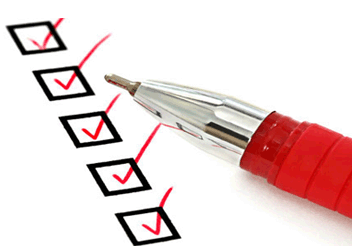
\includegraphics[scale=0.25]{images/requirement.png}
		\end{column}
	\end{columns}
\end{frame}

\subsection{Situazione attuale}
\begin{frame}{Situazione attuale}
	\only<1>
	{
		\begin{columns}
			\begin{column}{0.7\textwidth}
				Gestione ``semplicistica'' dei sorpassi:
				\begin{itemize}
					\item{\footnotesize{veicoli viaggiano a velocità costante}}
					\begin{itemize}
						\item{\scriptsize{pedone: 1200ms/10\% della strada}}
						\item{\scriptsize{auto: 500ms/10\% della strada}}
						\item{\scriptsize{bus: 800ms/10\% della strada}}
					\end{itemize}
					\item{\footnotesize{veicoli viaggiano in fila indiana}}
					\item{\footnotesize{sorpassi solamente tra veicoli di tipo differente}}
					\begin{itemize}
						\item{\scriptsize{scarsa fedeltà}}
						\item{\scriptsize{evento non segnalato}}
					\end{itemize}
				\end{itemize}
			\end{column}
			\begin{column}{0.3\textwidth}
				\centering
				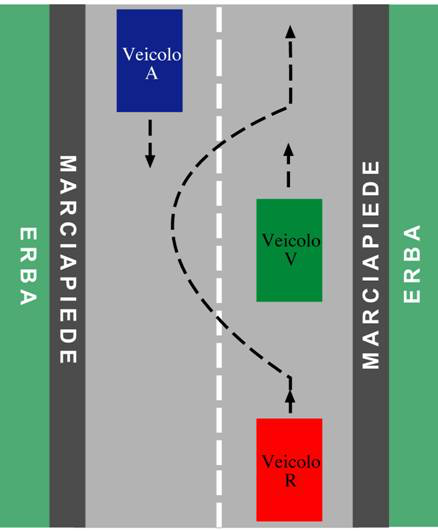
\includegraphics[scale=0.2,angle=-90]{images/overtaking.png}
			\end{column}
		\end{columns}
	}
	\only<2>
	{
		Esempio sorpasso tra automobile e pedone
		\centering
		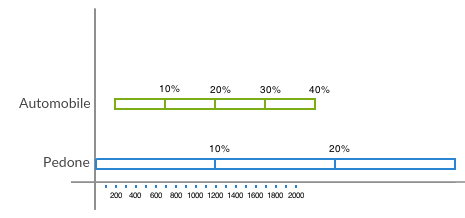
\includegraphics[scale=0.5]{images/timeline.png}
	}
\end{frame}

\subsection{Dove apportare le modifiche}
\begin{frame}{Dove apportare le modifiche}
	\only<1>
	{
		\centering
		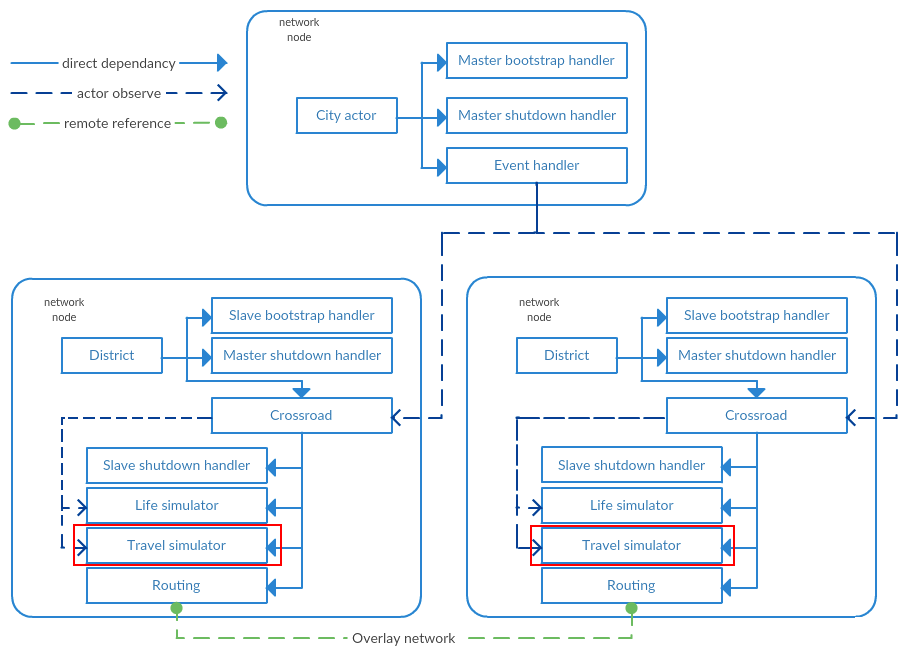
\includegraphics[scale=0.27]{images/overtakingIntervents.png}
	}
	\only<2>
	{
		\begin{columns}
			\begin{column}{0.7\textwidth}
				Interventi:
				\begin{itemize}
					\item{\footnotesize{spostare velocità di crociera dei veicoli}}
					\begin{itemize}
						\item{\scriptsize{fase di test -> campo statico in ogni veicolo}}
						\item{\scriptsize{produzione -> file di configurazione}}
						\item{\scriptsize{``getter'' di accesso in ogni veicolo}}
					\end{itemize}
					\item{\footnotesize{messaggi in ingresso inalterati}}
					\begin{itemize}
						\item{\scriptsize{startNewTrip}}
						\item{\scriptsize{progress}}
					\end{itemize}
					\item{\footnotesize{``lista dei transiti''}}
					\begin{itemize}
						\item{\scriptsize{mezzo}}
						\item{\scriptsize{percentuale strada percorsa}}
						\item{\scriptsize{evento pianificato}}
					\end{itemize}
					\item{\scriptsize{revisione algoritmo gestione messaggio ``progress''}}
				\end{itemize}
			\end{column}
			\begin{column}{0.3\textwidth}
				\centering
				
\includegraphics[scale=0.15]{images/need.png}
			\end{column}
		\end{columns}
	}
\end{frame}

\subsection{Algoritmo}
\begin{frame}{Algoritmo}
	\centering
	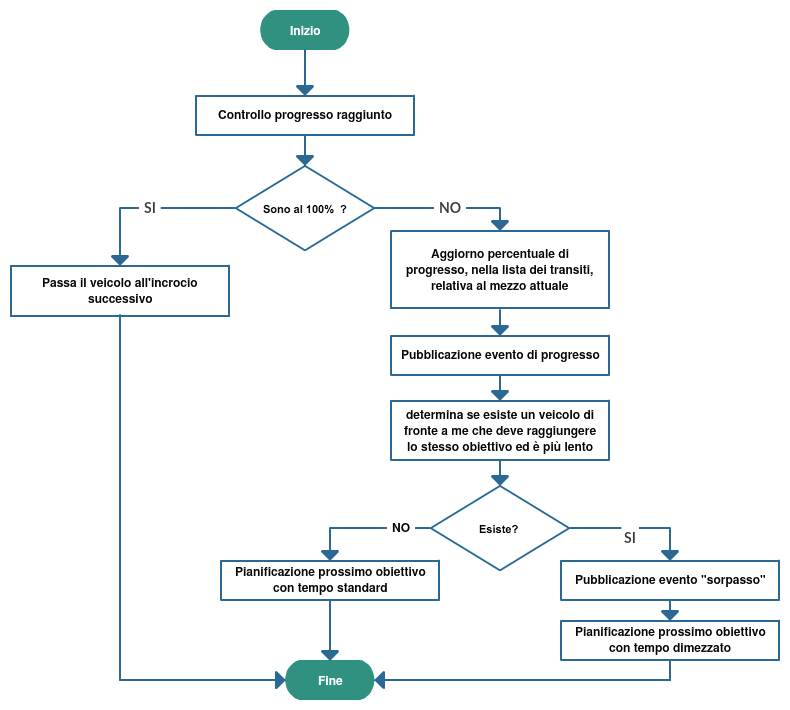
\includegraphics[scale=0.27]{images/algorithm.png}
\end{frame}

\subsection{Modello alternativo}
\begin{frame}{Modello alternativo}
	Per una simulazione più reale:
	\begin{itemize}
		\item{\footnotesize{necessarie più corsie per senso di marcia}}
		\begin{itemize}
			\item{\scriptsize{tanti sotto attori di ``TravelSimulator''}}
			\item{\scriptsize{un attore rappresenta una percentuale della strada}}
		\end{itemize}
		\item{\footnotesize{necessario un protocollo di comunicazione}}
		\begin{itemize}
			\item{\scriptsize{necessario accesso alla corsia con mutua esclusione}}
			\item{\scriptsize{deve ``chiedere'' l'accesso}}
		\end{itemize}
	\end{itemize}
	\begin{proof}[Modello ad attori \scriptsize{(ask statement)}]
		\scriptsize{Be careful when writing code that waits for immediate responses with ``ask' statement'. This causes your actor to block, which means that it can’t respond to anything else while it’s in this state. When you need to perform work like this, the mantra is, ``Delegate, delegate, delegate''. (cit. Akka Cookbook)}
	\end{proof}
\end{frame}